%%%%%%%%%%%%%%%%%%%%%%%%%%%%%%%%%%%%%%%%%%%%%%%%%%%%%%%%%%%%%%%%%%%


\documentclass[runningheads,a4paper]{llncs}
\usepackage{graphicx}
\usepackage{amssymb}
\usepackage{amsmath}
\setcounter{tocdepth}{3}
\usepackage{graphicx}
\usepackage{clrscode}
\usepackage{url}
\newcommand{\keywords}[1]{\par\addvspace\baselineskip
\noindent\keywordname\enspace\ignorespaces#1}
\makeatletter
    \newcommand\fcaption{\def\@captype{figure}\caption}
\makeatother
\begin{document}

\mainmatter
\title{Fusing Human Faces}
\author{Xianxiang Wang}
\institute{University of Science and Technology of China, 230031 Hefei, China\\
\url{kowo@mail.ustc.edu.cn}}
%\toctitle{Lecture Notes in Computer Science}
%\tocauthor{Authors' Instructions}
\maketitle


\begin{abstract}
Face fusion technology grows more important in recent years. In this paper, we propose an algorithm to fuse features of source face into target face. There are two main challenges in our task. The first challenge is how to rearrange facial features of target face properly according to source face. The second challenge is to keep hues and illumination information of target face as much as possible so that output face looks more photorealistic. Our algorithm contains two steps. First, we align two faces according to facial landmarks, which give us sizes, locations and distributions  of features of two faces, segment two faces into several triangles using Delaunay triangulation and warp the corresponding triangles of two faces into the same shape. Second, we reconstruct gradients for new face that we are going to generate. With one face image as target image and reconstructed gradients, we generate fused face by seamless clone. We propose an algorithm to reconstruct the new face gradients by preserving the weaker gradients of the target face. Our experiments show that proposed method preserves lots of illumination information and facial hues of target faces, which means output faces still look photorealistic.
\keywords{Face fusion, Facial landmarks, Delaunay triangulation, Seamless clone}
\end{abstract}


\section{Introduction}
These years, there has been a great need for face editing application. Someone would wonder what they look like if they have some face features from pop stars, and they may make their faces sharper through face editing application. While some other people want to know what they look like when they grow older. These tasks could be accomplished by face fusion. Progeny appearance prediction is a popular task lately. What the son of a young couple looks like when he grows up. It is attracting for many people, and this could also be accomplished by face fusion technology.

As we know, different faces have different features. Someone has a sharper face while the shapes of other faces are closer to square. There are many ways to build correspondences of two faces. In early years, hand-marked features of faces are used to build correspondences of two faces \cite{fbim}. Because of the lack of the technology to detect face features automatically, when we align two faces using this method, there are a lot of labour work to do. Lately, a five feature points based face morphing method \cite{mhf} was proposed. The five feature points are detected automatically. Then with these feature points, two faces could be warped and fused into one. In fact, five feature points are not enough to represent a face. When we use the sparse correspondences to generate new faces, the results are weird.

Given two faces, source face is the face that we want to use its features to influence other faces, while target face is the face waited to influenced. There are 68 facial landmarks detected by using Ensemble of Regression Trees \cite{fld} in our method. Thus we estimate the distributions of the features and the size of the face. Facial landmarks indicate face structures, while face gradients indicate face details. When we fuse two faces, first, we warp two faces to make sure the structures of two warped faces are the same. Here, we propose a method  to create a new set of landmarks by interpolating two groups of given landmarks. Then, we fuse the gradients of two faces. In order to maintain the hues and illumination information of the target face, we reconstruct the gradients for new faces by preserving the weaker gradients of the target face and fusing the stronger gradients of the two faces. Then, we recover the fused face by seamless clone \cite{pie}.

Our contributions can be summarized as follows. First, we propose a new method to fuse features of source face into target face. Second, we develop an algorithm to reconstruct gradients of fused face which keeps lots of facial hues and illumination information of target face, so the fused face looks more photorealistic. Third, we develop a user interface, for which users can decide how many features we want to fuse into target face from source face. 
\section{Related work}

In this section, we summarize existing face editing techniques that are related to our work.

<<<<<<< HEAD
\noindent\textbf{Face Morphing.} Face morphing is commonly referred as a smooth animated transformation of one digital face image to another.
In most cases, the background of the face image is pure in order to make us focus on transition itself.
\cxj{The morphing problem has nothing related with background. The background can be easily removed by face detection. }

Beier and Neely \cite{fbim} developed a user interface to build the correspondences of two faces by a group of line pairs.
The procedure of building correspondences of two faces is tedious and time-consuming. Besides, hand-marked features are not precise. After building correspondences, the corresponding pixels are linearly interpolated.
Wolberg \cite{wol} proposed a mesh-based method to build the correspondences of two faces.
=======
\noindent\textbf{Face Morphing.} Face morphing is commonly referred as a smooth animated transformation of one digital face image to another. 
In most cases, the background of the face image is pure in order to make us focus on transition itself. 
\cxj{The morphing problem has nothing related with background. The background can be easily removed by face detection. }

Beier and Neely \cite{fbim} developed a user interface to build the correspondences of two faces by a group of line pairs. 
The procedure of building correspondences of two faces is tedious and time-consuming. Besides, hand-marked features are not precise. After building correspondences, the corresponding pixels are linearly interpolated.  
Wolberg \cite{wol} proposed a mesh-based method to build the correspondences of two faces. 
>>>>>>> origin/master
The correspondences of two faces are referred as meshes instead of line pairs. Karungaru et al. \cite{mhf} detected five feature points as control points, then segmented face images into several triangles according to control points, next warped the face images according to corresponding triangles. These face morphing methods have a different way in building correspondences. Their aim is creating a seamless transition from one face to the other.

 In fact, face morphing is a seamless transition from one face image to the other. In other words, it is a transition of two images. It builds the correspondences of two faces, but not adjusts the sizes and the locations of two faces. It warps two images according to the correspondences and interpolates two warped images to generate intermediate images. So the intermediate images of the transition are not photorealistic. Our algorithm adjusts  the sizes and the locations of two faces. It operates only on two faces but not the whole images, and preserves lots of illumination information and facial hues of the target face. So the result of our algorithm is a photorealistic edited target face but not a transition of two images.

\noindent\textbf{Face Swapping.} Face swapping is also known as face replacement, which transfers a face from a source photo onto a face appearing in a target photo in order to generate a new genuine face.

<<<<<<< HEAD
The most early work for face swapping is \cite{exchface}. But the results are not that photorealistic. Later, the results are better \cite{de1,de2,de3,de4} and mainly used for deidentification. The main problem for face swapping is pose variation.
Many techniques solve this problem by using a 3D model \cite{3d1,de3,onseg}. Nirkin et al. \cite{onseg} transferred the face from source image onto target image using a 3D face model. They first detected facial landmarks that are used to establish 3D pose and facial expression for 3D face shape. Then they used a Fully Connected Network to segment the visible parts of faces from their contexts and occlusions. At last, source face is blended-in with the target context by using image seamless clone \cite{pie}. However, this step would fail when blending very different facial hues. Korshunova et al. \cite{faceswapping} proposed a network to generate a source face that could replace the face in the target image. The network only generate faces of the same type. For example, the net named CageNet only generate the face of Nicolas Cage. Those two methods mentioned above may greatly change the lightning condition of the face on the target image because they just transferred the source face onto the target image, but not contained any information of the target face. Bitouk et al. \cite{autorep} presented a system for automatic face replacement in images. Given a target face image, the system would retrieve a face with similar pose, lightning and color condition, then use such a face to replace the face on the target image. The limitation of this method is clear. The source face must have a similar pose and lightning condition with the target face.
%
The main difference between face swapping and our task is that we want to keep some features of the target face but not to replace the target face with the source face. In fact, how to fuse the features of the source face into the target face is our main consideration.
\cxj{So what is the difference between face fusion and face morphing?}
=======
The most early work for face swapping is \cite{exchface}. But the results are not that photorealistic. Later, the results are better \cite{de1,de2,de3,de4} and mainly used for deidentification. The main problem for face swapping is pose variation. 
Many techniques solve this problem by using a 3D model \cite{de3,3d1,onseg}. Nirkin et al. \cite{onseg} transferred the face from source image onto target image using a 3D face model. They first detected facial landmarks that are used to establish 3D pose and facial expression for 3D face shape. Then they used a Fully Connected Network to segment the visible parts of faces from their contexts and occlusions. At last, source face is blended-in with the target context by using image seamless clone \cite{pie}. However, this step would fail when blending very different facial hues. Korshunova et al. \cite{faceswapping} proposed a network to generate a source face that could replace the face in the target image. The network only generate faces of the same type. For example, the net named CageNet only generate the face of Nicolas Cage. Those two methods mentioned above may greatly change the lightning condition of the face on the target image because they just transferred the source face onto the target image, but not contained any information of the target face. Bitouk et al. \cite{autorep} presented a system for automatic face replacement in images. Given a target face image, the system would retrieve a face with similar pose, lightning and color condition, then use such a face to replace the face on the target image. The limitation of this method is clear. The source face must have a similar pose and lightning condition with the target face. 
%
The main difference between face swapping and our task is that we want to keep some features of the target face but not to replace the target face with the source face. In fact, how to fuse the features of the source face into the target face is our main consideration. 
\cxj{So what is the difference between face fusion and face morphing?}
>>>>>>> origin/master

\section{Face Fusion Algorithm}
\label{sec:algorithm}

Given a source face image $I_s$ and a target face image $I_t$, our goal is to generate a new face image $I_f$ which fuses the facial features of the two faces into a natural-looking face.
Our method consists of two steps: (1) \emph{geometric alignment}, which re-arranges the facial landmarks of the target face according to the source face, and (2) \emph{appearance fusion}, which fuses two faces in the gradient domain. Fig.~\ref{fig:pipeline} shows the pipeline of our approach.




\comments{
It is necessary to calculate the location and the size of the facial part from each face image. With the help of the facial landmarks \cite{fld}, it is quick to perform this step. But only knowing the location and the size of two faces is not enough. We need to know where are the eyes, nose and other parts of two faces. Different faces have different face features, some people have a big nose while others with a small one. Some people's nose is closer to eyes while others' nose is farther to eyes. Still, with the help of facial landmarks, we know exactly the distribution of face features.


By aligning two faces, we know the features on one face and their corresponding features on the other face. Then, we fuse two faces from parts to parts.
}

\begin{center}
    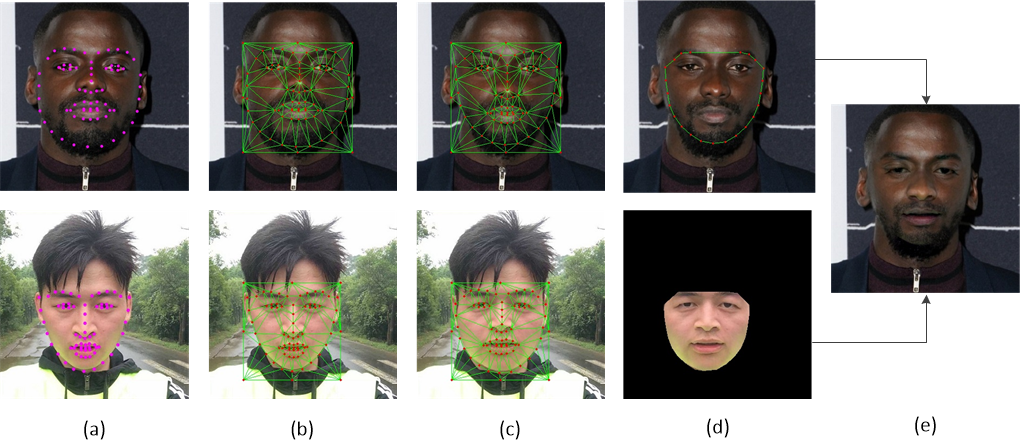
\includegraphics[width=4.8in]{images/pipeline.png}
    \fcaption{Pipeline of our approach. (a) Perform facial landmark detection on two faces. (b) Triangulate two faces according to the facial landmarks. (c) Calculate new facial landmarks by interpolating two groups of facial landmarks, warp two faces according to the new facial landmarks. (d) Reconstruct gradients on facial part for fused face . (e) Fuse features of source face into target face by seamless cloning. \cxj{Choose two figures that are more beautiful. Mark the source and target image.}}
    \label{fig:pipeline}
\end{center}

\subsection{Face alignment}


\mdf{While the two face areas are different in scale, position, and orientation in $I_s$ and $I_t$, we first align the two faces according to their facial landmarks. }
%
There are many techniques to detect facial landmarks \cite{fld2,fld3,fld4,fld}. We adopt \cite{fld}. It is an much faster method exist;
%It is implemented in Dlib.
\cxj{Why do you choose this method?}

In Fig.~\ref{fig:pipeline}(a), with the landmarks of two faces, the bounding boxes of two faces are calculated. But two bounding boxes can not be directly compared.
We reshape the bounding boxes of two faces into square by stretching the shorter side of bounding boxes and get bounding squares of two faces.
With the bounding squares of two faces, we know the sizes of two faces.
\cxj{Why don't you directly compute the transformation between two bounding boxes?}
%
%
Before we triangulate a face according to facial landmarks, we need make sure that the transition from the background to the face is natural. If we interpolate two groups of facial landmarks directly, the profile of the interpolated facial landmarks would be different from the facial landmarks of the target face.
\cxj{why do you have to consider the background area?}
%
So we add eight points into the facial landmarks to help triangulate the faces. In Fig.~\ref{fig:face-warpping}(b), the eight points lie on the boundary of a square. The square is generated by enlarging the bounding square of the face. Four points are on the corners of the square and the others are on the mid points of sides of the square.
%
The center point and the side length of bounding square of source face are denoted as $\mathbf{c}_s$ and $l_s$.
The center point and side length of bounding square of target face are denoted as $\mathbf{c}_t$ and $l_t$.
%
The indexes of facial landmarks on the face denoted as $i \in \{1...N\}$, $N$ is the number of facial landmarks.
For each point $\mathbf{p}_s$ inside the bounding square of source face, we calculate its corresponding location on the target face $\vb{p}_t$ by following mapping function:
%
\begin{equation}
\label{eq:trans-point}
\vb{p}_t=\frac{l_t}{l_s}(\vb{p}_s-\vb{c}_s) + \vb{c}_t.
\end{equation}

The facial landmarks we need to triangulate on the source face and the target face are denoted as $\vb{F_{s}}$(the red points on the face image in second row of Fig.~\ref{fig:pipeline}(b)) and $\vb{F_{t}}$(the red points on the face image in first row of Fig. 1(b)) respectively.
The facial landmarks of the output face are denoted as $\vb{F_n}$. It can be calculated by interpolating $\vb{F_s}$ and $\vb{F_t}$. With these new facial landmarks, we can create a new face structure. For each point in $\vb{F_s}$, $\vb{F_t}$ and $\vb{F_n}$, they are denoted as $\vb{F}_{\vb{s}_i}$, $\vb{F}_{\vb{t}_i}$ and $\vb{F}_{\vb{n}_i}$ respectively.

\begin{equation}
\label{eq:inp-point}
\vb{F}_{\vb{n}_i} = \alpha \cdot f(\vb{F}_{\vb{s}_i}) + (1-\alpha) \cdot \vb{F}_{\vb{t}_i},
\end{equation}

where $\alpha$ controls which face structure we prefer more. If $\alpha$ is small, the new face structure would look more like the target face. It means that the profile of the new face and the distribution of the new face features would look more like the target face.

After triangulating two faces according to $\vb{F_s}$ and $\vb{F_t}$ using Delaunay Triangulation, we get two sets of triangles from the source face and the target face, denoted as $\vb{T_s}$ and $\vb{T_t}$. The corresponding triangles of two faces are not of the same shape because of different facial landmarks. What we need to do is to make sure the shape of corresponding triangles of two faces are the same. We warp the triangles in $\vb{T_{t}}$ one by one to the $\vb{T_{n}}$. Then we warp $\vb{T_s}$ to $\vb{T_n}$ in a similar way.
\cxj{1. How to warp the triangular mesh? Warping each triangle independently?}

In Fig.~\ref{fig:pipeline}(c), the source face and the target face are warped according to an common interpolated mesh. The sizes and the locations of their bounding squares are different at each face image, but the shapes of the corresponding triangles of two faces are the same.
\cxj{Given two meshes, there should be just one transformation to alignment.}

After warping two faces, we have two faces of the same structures and the same distributions of face features. But the sizes and the locations of their bounding squares are different. We extract the bounding square area of the source face, scale and translate the area to the same size and location of the bounding square of the target face. The extracted face witch is translated and resized is shown in Fig.~\ref{fig:face-warpping}(b).

As we can see from the Fig.~\ref{fig:face-warpping}, the triangles of the source face and the target face are exactly at the same location and of the same shapes and sizes. The purpose of our task is to fuse the features of the source face into the target face. So we need to know the profile of the source face. In Fig.~\ref{fig:face-warpping}(c), the yellow outline is generated from the facial landmarks. What we want is that all the pixels inside the yellow outline are from the face. In fact, some pixels may come from the background. So we get the blue outline by shrinking the profile a little. Inside the blue outline, all the pixels are from the facial part. The area inside the blue outline is $\Omega$, where $\Omega$ stands for the facial part we are going to fuse.

\cxj{This should be in the face alignment part which computes the geometric transformation.}


\begin{center}
    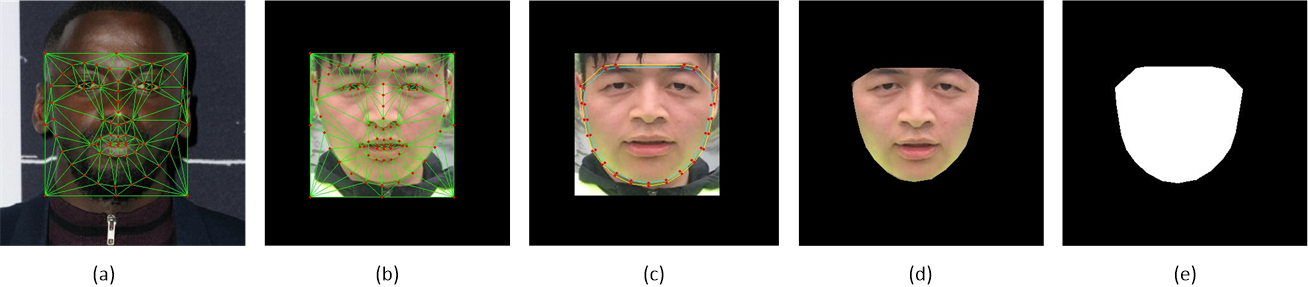
\includegraphics[width=4.8in]{images/extract.png}
    \fcaption{(a) The target face warped according to $\vb{F_n}$. (b) The warped source face after being translated and scaled. (c) Yellow outline is generated from the landmarks of the warped source face, light blue outline is shrank a little from the yellow profile. (d) Facial part of the warped source face that inside $\Omega$. (e) Facial mask. \cxj{Why do you need to show two outlines in (c)? They should be the same.}}
    \label{fig:face-warpping}
\end{center}


\subsection{Gradient-based Fusion}
\label{sec:fusion}

The target face and the source face are shown in Fig.~\ref{fig:face-warpping}(a) and Fig.~\ref{fig:face-warpping}(b). We fuse the gradients of two faces, recover the face from the fused gradients by seamless clone.

The gradients of the source face is denoted as $g_s$. The gradients of target face is denoted as $g_t$. There are three ways we tried to construct the guidance field.

For the first way, the guidance field $g_1$ is generated  by linearly combinating $g_s$ and $g_t$:

\begin{equation}
\label{eq:gradient-linear}
g_1 = \beta g_s+(1-\beta) g_t.
\end{equation}

For the second way, at each point in $\Omega$, guidance field $g_2$ retain the stronger gradients in $g_s$ or in $g_t$:

\begin{equation}
\label{eq:gradient-mixed}
for\ all\ \vb{x} \in \Omega, g_2(\vb{x})=\left\{
\begin{aligned}
g_s(\vb{x}) &&{if |g_s(\vb{x})|>|g_t(\vb{x})|}\\
g_t(\vb{x}) &&{else}\\
\end{aligned}
\right.
\end{equation}

For the third way, we define $g_3$ by linearly combination of $g_d$ and $g_t$:

\begin{equation}
\label{eq:gradient-shed}
g_3 = \beta \cdot g_d+(1-\beta) \cdot g_t,
\end{equation}


where $g_d$ is:

\begin{equation}
\label{eq:gradient-mixed-sub}
for\ all\ \vb{x} \in \Omega, g_d(\vb{x})=\left\{
\begin{aligned}
g_t(x) &&{if \ |g_s(\vb{x})|< \theta_1 \ and \ |g_t(\vb{x})|< \theta_2}\\
g_s(x) &&{else}\\
\end{aligned}
\right.
\end{equation}


$g_d$ contains the stronger gradients of the $g_s$ and weaker gradients of $g_t$. If $g_s(\vb{x})$ is smaller than the threshold $\theta_1$ and $g_t(\vb{x})$ is smaller than the threshold $\theta_2$, then $g_d(\vb{x})$ keeps the gradient from $g_t$ at point $x$. So it contains main features of the source face and the part of the lightning condition of the target face. Fig.~\ref{fig:shed}(a) and Fig.~\ref{fig:shed}(b) are facial parts of the target face and the source face. They share the same profile and distribution of features, Fig.~\ref{fig:shed}(c) shows which parts of $g_d$ are come from $g_t$ or $g_s$. For all $\vb{x} \in \Omega$ and for each channel, if $g_d(\vb{x})$ is come from $g_s(\vb{x})$, then the corresponding part in Fig.~\ref{fig:shed}(c) is brighter.

\cxj{All these ways to create gradient field can be found in \cite{pie}, you only need one sentence "the gradient field is calculated in the same way with \cite{pie}."}

Finally, we use $g$ to recover the face we want on the target face image by seamless clone.
\begin{center}
    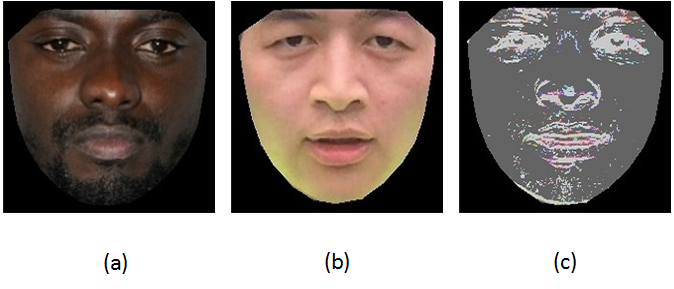
\includegraphics[width=3in]{images/labelmasks.png}
    \fcaption{(a) Facial part of target face. (b) Facial part of the source face. (c) A mask indicates which part of $g_d$ are come from $g_s$ or $g_t$.}
    \label{fig:shed}
\end{center}

\section{Experiments}


First, we compare the results of different face gradient reconstruction. 
Then we conduct several experiments to show that how parameters effect the results.
\cxj{To validate the proposed method, comparison with related approaches is also needed.}


\subsection{Gradient field construction}
\begin{center}
    \includegraphics[width=4.8in]{images/3cmp.png}
    \fcaption{The effects of different gradient reconstruction: (a) Source face image. (b) Target face image. (c) Fusing face by linearly combining the gradients of two faces \cxj{according to Eq.~\ref{eq:gradient-linear}?} (d) Fusing face by keeping the larger gradients of two faces. \cxj{Eq.?} (e) Fusing face through weaker gradient preserving method.\cxj{Eq.?}}
\end{center}

Fig. 4 shows the effects of different face gradient reconstruction. From Fig. 4(c), we can see that direct linear combination of  gradients of two faces could bring too much illumination from the source face into the target face, which makes face look very unnatural. 
\cxj{What happens if the target image is lighter?}
%
If we kept the stronger gradients of two faces, the lightning condition of the target face would be strongly broken. 
%
More importantly, we can't control how much features we are going to fuse from the source face into the target face. 
In Fig. 4(e), the lightning condition and facial hues is closest to the target face image among all the results. 
\cxj{Fusing face through weaker gradient?}
%
When we reconstruct gradients using the proposed algorithm, we only keep the stronger gradients of the source face, which means the main features of the source are preserved.

\subsection{Parameters of face fusion}

 For our task, there are four parameters we can adjust, they are $\alpha$, $\beta$, $\theta_1$, $\theta_2$. $\alpha$ controls the structure of human faces, in other words, it controls the profile and the distribution of features of human faces. 
 $\beta$ controls the details of human faces, like wrinkles and textures. 
 \cxj{$\beta$ is just a linear combination weight. How can it control face details? It only controls how much it looks like the source image. }
 %
 With $\alpha$ and $\beta$, we can control how much content we want to fuse from source face into target face. 
 %
 If the gradients of source face is weaker than $\theta_1$ and the gradients of target face is weaker than $\theta_2$, then we retain the gradients of the target face. 
 Otherwise, we keep the gradients of the source face.

Fig. 5 shows how $\alpha$ effects the fused results, $\beta = 0.5$, $\theta_1 = 10$, $\theta_2 = 15$. As the $\alpha$ grows bigger, the distribution of face features of fused face is more like the source face.

\begin{center}
    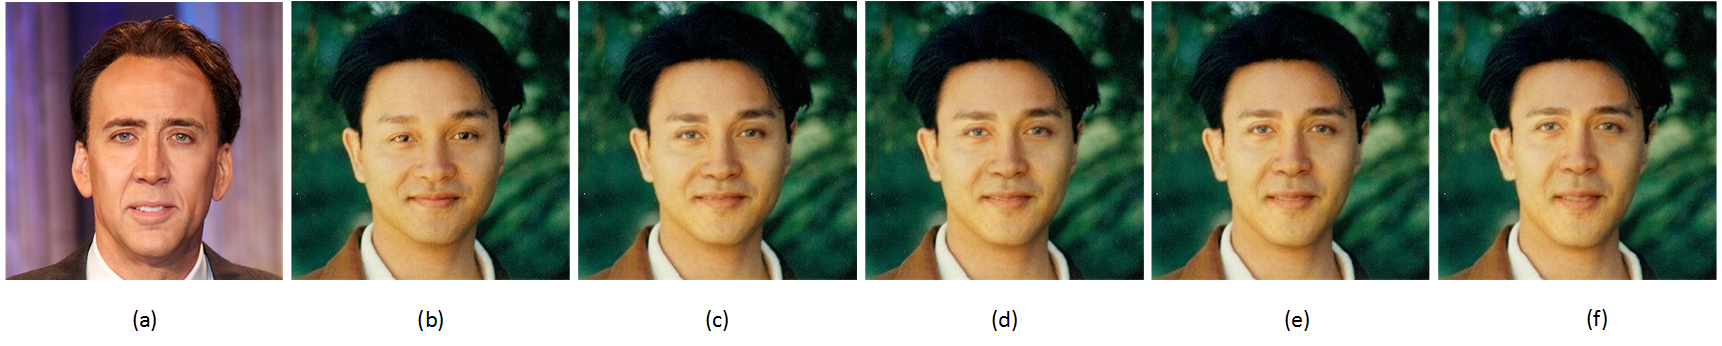
\includegraphics[width=4.8in]{images/pro.png}
    \fcaption{(a) Source face. (b) Target face. (c) Fused face, $\alpha = 0.2$. (d) Fused face, $\alpha = 0.4$. (e) Fused face, $\alpha = 0.6$. (f) Fused face, $\alpha = 0.8$.}
\end{center}

Fig. 6 shows how $\beta$ effects the fused result. $\alpha = 0.5$, $\theta_1 = 10$, $\theta_2 = 15$. As the $\beta$ grows bigger, the fused result has more details from source face.

\begin{center}
    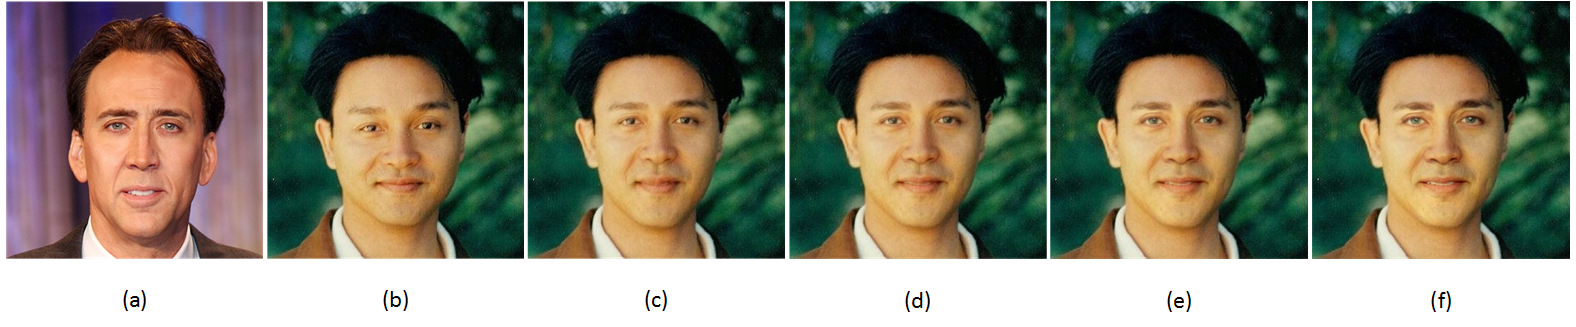
\includegraphics[width=4.8in]{images/detail.png}
    \fcaption{(a) Source face. (b) Target face. (c) Fused face, $\beta = 0.2$. (d) Fused face, $\beta = 0.4$. (e) Fused face, $\beta = 0.6$. (f) Fused face, $\beta = 0.8$.}
\end{center}

If we want to only keep main features of source face, we could only retain stronger gradients of the source face, Fig. 7 shows that the fused results are more natural as more weaker gradients of the source face are been dropped. $\alpha = 0.5$, $\beta = 0.5$, $\theta_2 = 40$. The weaker gradients carry too much illumination information and facial hues of the source face, when these gradients are brought into the fused results, the results become very unnatural.

\begin{center}
    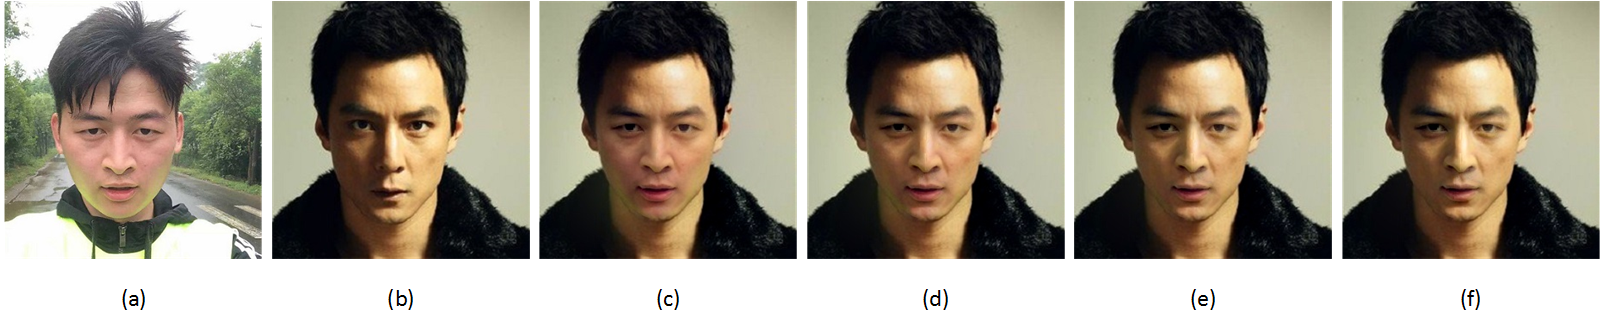
\includegraphics[width=4.8in]{images/thd1.png}
    \fcaption{(a) Source face. (b) Target face. (c) Fused face, $\theta_1 = 2$. (d) Fused face, $\theta_1 = 4$. (e) Fused face, $\theta_1 = 6$. (f) Fused face, $\theta_1 = 8$.}
\end{center}

When we fuse the main features of source face into target face, somehow, we need to erase the main features of target face. In fact, we want to keep the illumination information of the target face, both the weaker gradients of source face and weaker gradients of target face are preserved. For Fig. 8, it shows the experiment on $\theta_2$,  $\alpha = 0.5$, $\beta = 0.5$, $\theta_1 = 10$, when the $\theta_2$ grows bigger, more stronger gradients are preserved. As we can see, more shadows are preserved.

\begin{center}
    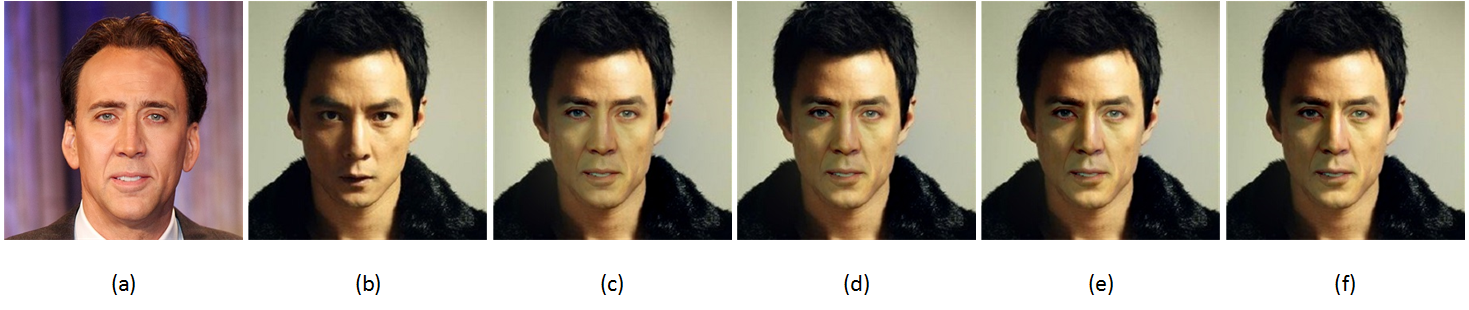
\includegraphics[width=4.8in]{images/thd2.png}
    \fcaption{(a) Source face. (b) Target face. (c) Fused face, $\theta_2 = 10$. (d) Fused face, $\theta_2 = 20$. (e) Fused face, $\theta_2 = 30$. (f) Fused face, $\theta_2 = 40$.}
\end{center}

Although our work are not aiming at face swapping task, we still could create similar effects by setting $\beta = 1$.
\cxj{$\alpha$ should be 1 also.}
% 
This means we almost preserving all the gradients of source faces, but only keep part of weaker gradients of target faces. We compare our results and the work of Korshunova et al. \cite{faceswapping}. In Fig. 9, the source face of all the results is from Fig. 8(a), we can see that our results keep more illumination information and facial hues of target faces which makes our results more natural. But in Fig. 9(c), our result fail to catch the lightning condition of the target face from a high level, this is where we need improve.

\begin{center}
    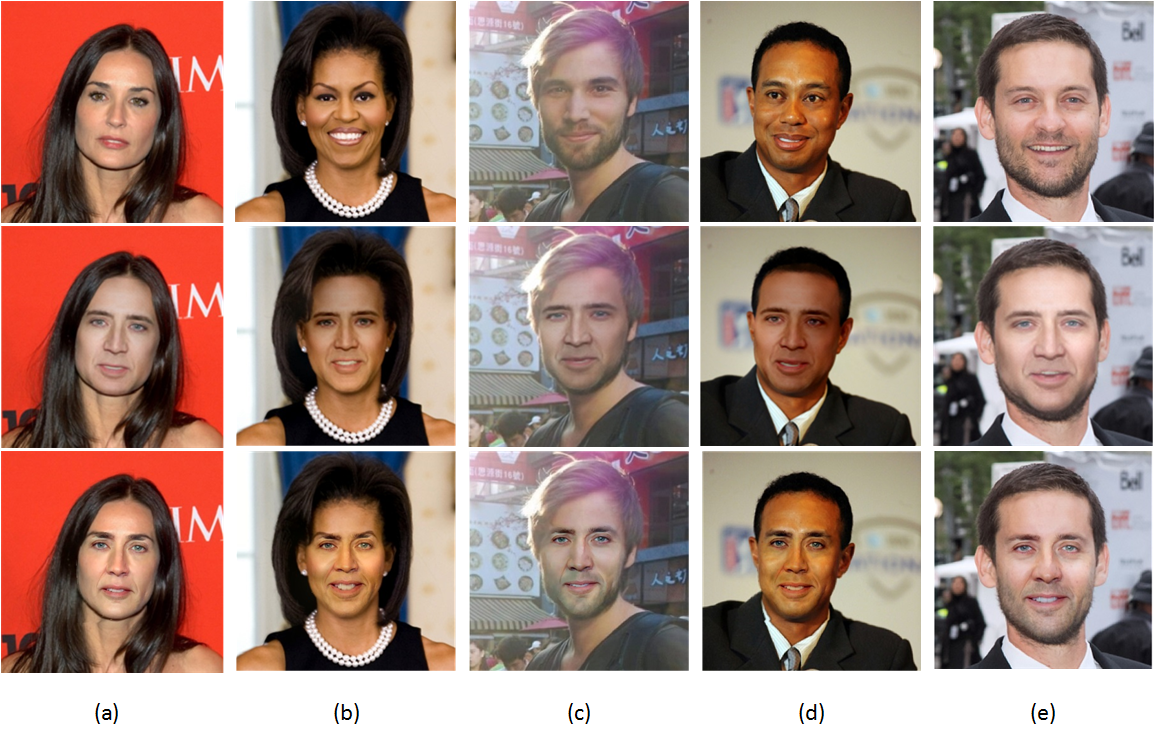
\includegraphics[width=4.8in]{images/vs.png}
    \fcaption{The first row are the original target face, the second row are the results of Korshunova et al., the third row are our results. Our algorithm preserves more illumination information and facial hues of target face.}
\end{center}

In Fig. 10, as $\alpha$ and $\beta$ grow bigger, the output faces have more features from the source face.

\begin{center}
    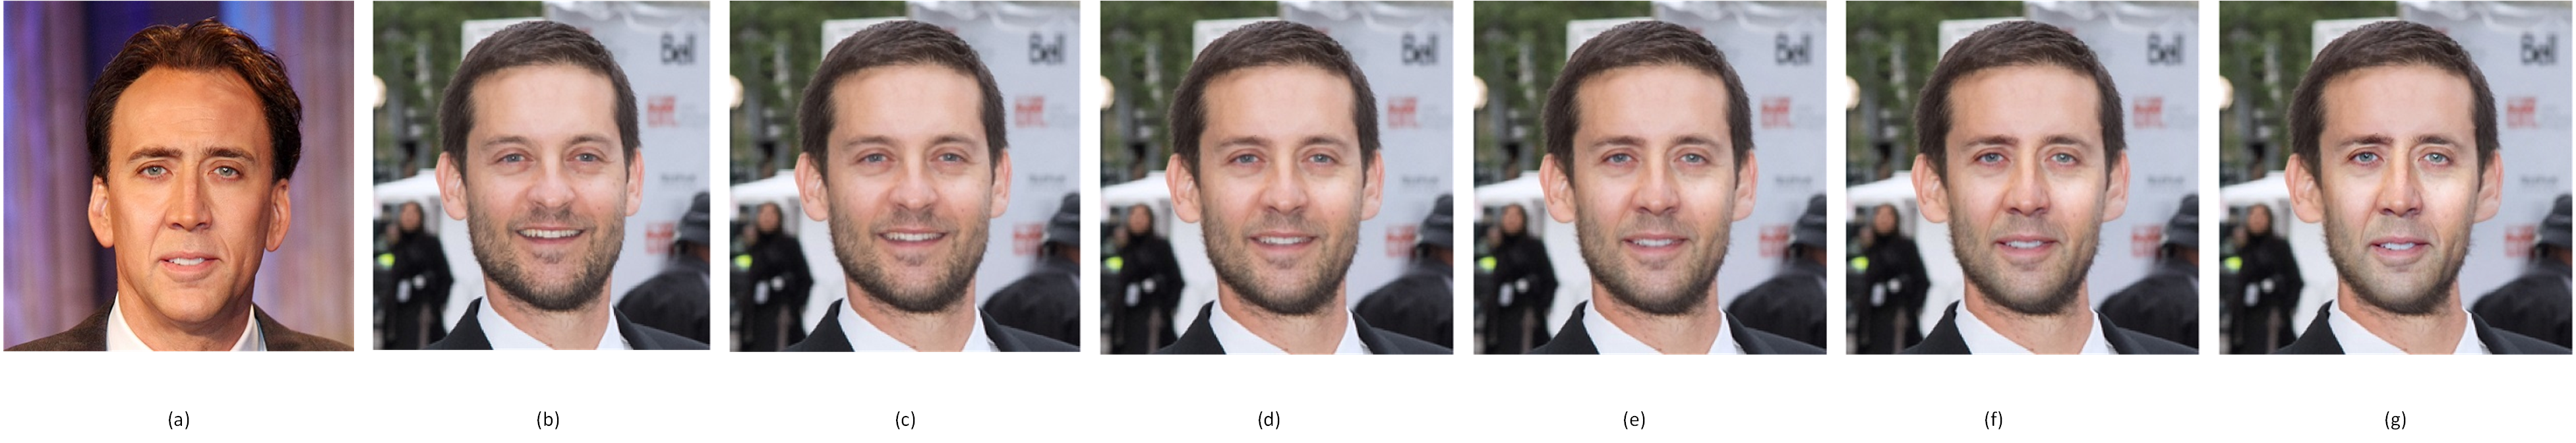
\includegraphics[width=4.8in]{images/trans.png}
    \fcaption{(a) Source face. (b) Target face. (c) Fused face, $\alpha = 0.2$, $\beta = 0.2$. (d) Fused face, $\alpha = 0.4$, $\beta = 0.4$. (e) Fused face, $\alpha = 0.6$, $\beta = 0.6$. (f) Fused face, $\alpha = 0.8$, $\beta = 0.8$. (g) Fused face, $\alpha = 1$, $\beta = 1$. \cxj{Put the parameters under each image.}}
\end{center}

\section{Conclusions}

We developed a face fusion method that automatically fuses features of source face into target face. When we consider fusing human faces, there are two parts we are going to fuse, one is face structures, the other is face details. The 68 facial landmarks are enough to align two faces precisely. The illumination of source face might pollute target face. But the method we proposed preserves as much illumination information as possible while decreasing the influence of the illumination of the source face. At mean time, we developed a user interface for letting users control how many features they want from the source face to fuse into the target face. The limitation of our method is clear, we have small tolerance to pose variation. Once two faces are in different poses, warping faces changes the original distributions of face features. 
\begin{thebibliography}{4}

\bibitem{fbim} Beier, T., and Neely, S.: Feature-based image metamorphosis. In: ACM SIGGRAPH Computer Graphics, Vol. 26, No. 2, pp. 35-42 (1992)
\bibitem{autorep}Bitouk, D., Kumar, N., Dhillon, S., Belhumeur, P., Nayar, S. K.: Face swapping: automatically replacing faces in photographs. ACM Transactions on Graphics (TOG), 27(3), 39. (2008). doi: 10.1145/1399504.1360638
\bibitem{exchface}Blanz, V., Scherbaum, K., Vetter, T., Seidel, H. P.: Exchanging faces in images. In: Computer Graphics Forum, Vol. 23, No. 3, pp. 669-676 (2004). doi: 10.1111/j.1467-8659.2004.00799.x
\bibitem{fld4}Cao, X., Wei, Y., Wen, F., Sun, J.: Face alignment by explicit shape regression. In: International Journal of Computer Vision. (2014). doi: 10.1007/s11263-013-0667-3
\bibitem{de1}De La Hunty, M., Asthana, A., Goecke, R.: Linear facial expression transfer with active appearance models. In: International Conference on Pattern Recognition (ICPR) (2010). doi: 10.1109/ICPR.2010.923
\bibitem{fld}Kazemi, V., and Sullivan, J.: One millisecond face alignment with an ensemble of regression trees. In: Proc. IEEE Conf. Computer Vision and Pattern Recognition (CVPR), pp. 1867-1874 (2014). doi: 10.1109/CVPR.2014.241
\bibitem{mhf}Karungaru, S., Fukumi, M., Akamatsu, N.: Morphing Human Faces: Automatic Control Points Selection And Color Transition. In: International Conference on Computational Intelligence, pp. 224-227 (2004)
\bibitem{faceswapping}Korshunova, I., Shi, W., Dambre, J., Theis, L.: Fast face-swap using convolutional neural networks. arXiv preprint arXiv:1611.09577. (2016)
\bibitem{3d1}Lin, Y., Lin, Q., Tang, F., Wang, S.: Face replacement with large-pose differences. In: Proceedings of the 20th ACM international conference on Multimedia. (2012). doi: 10.1145/2393347.2396426
\bibitem{de3}Lin, Y., Wang, S., Lin, Q., Tang, F.: Face swapping under large pose variations: A 3D model based approach. In: International Conference on Multimedia and Expo (ICME), pp. 333-338 (2012)
\bibitem{de4}Mosaddegh, S., Simon, L., Jurie, F.: Photorealistic Face de-Identification by Aggregating Donors�� Face Components. In: Asian Conference on Computer Vision, pp. 159-174 (2014). doi: 10.1007/978-3-319-16811-1_11

\bibitem{onseg}Nirkin, Y., Masi, I., Tran, A. T., Hassner, T., Medioni, G.: On Face Segmentation, Face Swapping, and Face Perception. arXiv preprint arXiv:1704.06729. (2017)
\bibitem{pie}P��rez, P., Gangnet, M., Blake, A.: Poisson image editing. In: ACM Transactions on Graphics (TOG), Vol. 22, No. 3, pp. 313-318 (2003). doi: 10.1145/882262.882269


\bibitem{fld3}Ren, S., Cao, X., Wei, Y., Sun, J.: Face alignment at 3000 fps via regressing local binary features. In: Proceedings of the IEEE Conference on Computer Vision and Pattern Recognition.(2014). doi: 10.1109/CVPR.2014.218
\bibitem{de2}Ross, A., Othman, A.: Visual cryptography for biometric privacy. In: IEEE transactions on information forensics and security.(2011). doi: 10.1109/TIFS.2010.2097252


\bibitem{wol}Wolberg, G.: Image morphing: a survey. In: The visual computer, 14(8), 360-372 (1998). doi: 10.1007/s003710050148



\bibitem{fld2}Xiong, X., and De la Torre, F.: Supervised descent method and its applications to face alignment. In: Proceedings of the IEEE conference on computer vision and pattern recognition.(2013). doi: 10.1109/CVPR.2013.75





\end{thebibliography}






\end{document}
